\section{Project-Based Comparison}\label{sec:proj_eval}

This section compares the performance of AmbientTalk, LIME, and SpatialViews in a regular wired LAN and in a MANET context using EXata.

The wired LAN environment provides a nearly ideal network in which the cost of communication is very low, there is little contention for the communication channel, all nodes are connected directly to each other, and collisions are minimal. By minimizing these factors, it is possible to focus the experiment results on the overhead of the programming environments. In these experiments, all nodes were directed connected to a 100Mb/s switch, providing essentially an independent, one hop channel for each pair of nodes

The results using EXata more accurately reflect the MANET environment. For these experiments, all communication was performed through EXata, which emulated an 802.11 ad hoc wireless network with an available bandwidth of 11Mb/s.

\begin{figure}
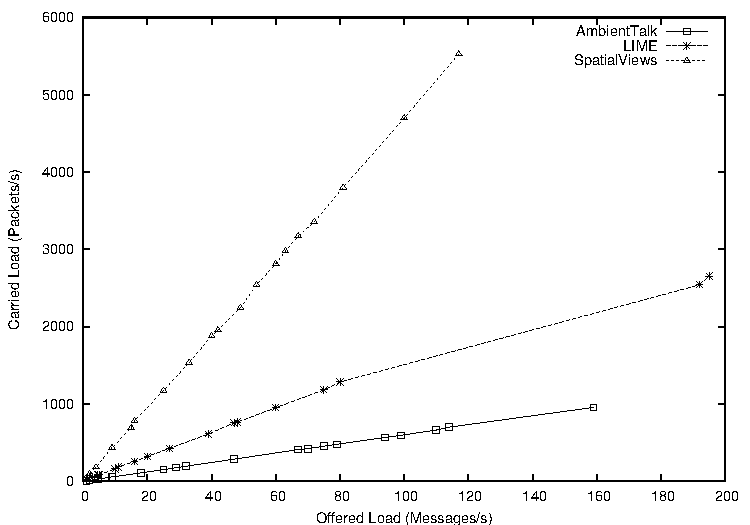
\includegraphics[scale = .70]{figures/overhead-wired.pdf}
\caption{Communication Overhead with Wired Links}
\label{fig:overhead-wired}
\end{figure}

\begin{figure}
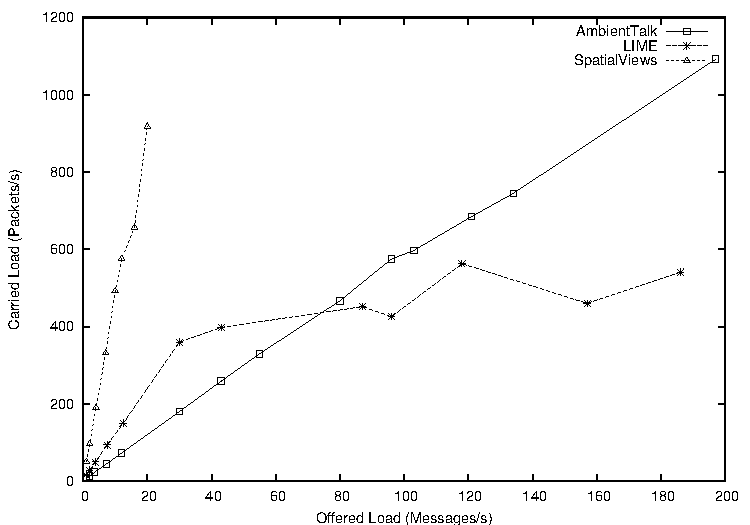
\includegraphics[scale = .70]{figures/overhead-qualnet.pdf}
\caption{Communication Overhead with Simulated Wireless Links}
\label{fig:overhead-qualnet}
\end{figure}

\subsection{Experimental Results}


\subsubsection{Communication Overhead}

AmbientTalk, LIME, and SpatialViews use very different messaging systems. This experiment demonstrates the overhead for each using a client-server setup as the simplest base case. Messages are sent out from the sever to the client at an increasing rate. The number of IP packets generated by doing so include control and discovery packets. Each node is within wireless range of the others so all communication is performed over single hop routes. Figure~\ref{fig:overhead-qualnet} and Figure~\ref{fig:overhead-wired} show the results from wired LAN and QualNet, respectively.

AmbientTalk has the lowest overhead, as it is simply performing a method call on a remote object and there is no return value. LIME requires some communication to alert merged tuple spaces of the messages' presence and then more communication to actually transfer the tuple. SpatialViews shows the highest amount of overhead, which is expected since it is migrating code and data to communicate a simple message. 

Although the results were similar in the wired LAN and EXata, the performance of SpatialViews was considerably slower, peaking at 20 msgs/s, while in the wired LAN it was possible to reach 117 msgs/s. This is due to contention for the wireless channel. It is also worth considering that LIME and AmbientTalk use asynchronous messages while SpatialViews uses a blocking synchronous message send. This allows LIME and AmbientTalk to take advantage of system level buffers, while SpatialViews cannot.

\begin{figure}
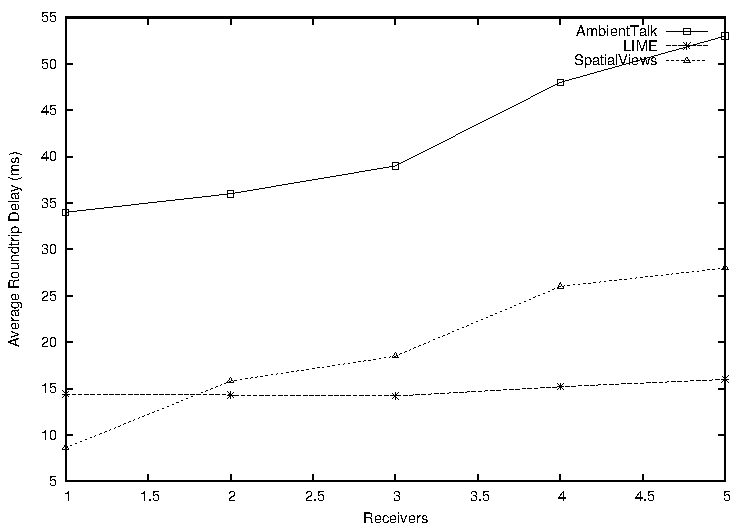
\includegraphics[scale = .70]{figures/multicast-wired.pdf}
\caption{Group Communication with Wired Links}
\label{fig:multicast-wired}
\end{figure}

\begin{figure}
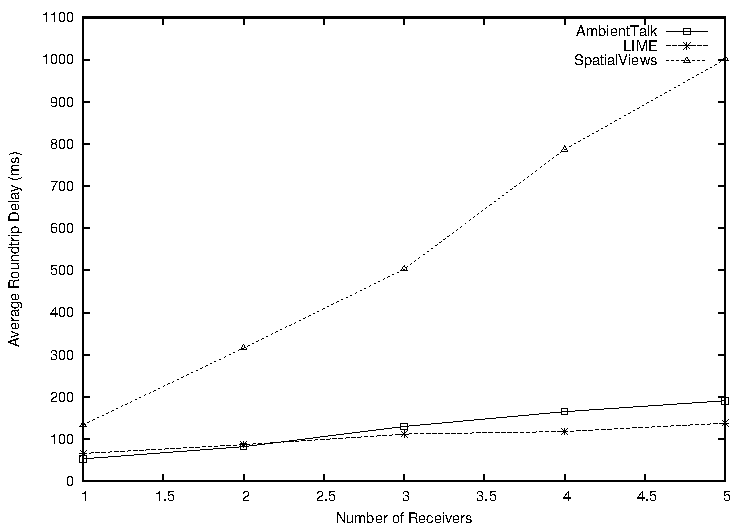
\includegraphics[scale = .70]{figures/multicast-qualnet.pdf}
\caption{Group Communication with Simulated Wireless Links}
\label{fig:multicast-qualnet}
\end{figure}


\subsubsection{Group Communication}

In this experiment we consider the common situation where one node needs to request information from the rest of the network and then collect the results, with increasing numbers of receivers. The application sends out a message then measures the time elapsed for responses.  For SpatialViews, this involves visiting each node and that node then visiting the sending node. The AmbientTalk version uses an omnihandle, as in the chat application, to broadcast the handle of the sender and then the receivers use the handle to send a return message. For LIME, each message is sent as a tuple, to which the receivers send a response tuple. Again, the network is set up so that no node is farther than one hop from any other node. Figures~\ref{fig:multicast-qualnet} and ~\ref{fig:multicast-wired} show the results.

In the wired LAN, LIME shows the least variation as the number of receivers increases. This is because the sender writes out a single tuple and each receiver can respond independently and in parallel. SpatialViews slows down considerably as the number of receivers increases, since SpatialViews visits each receiver in turn and waits on a response before continuing. The delay for AmbientTalk is the highest but does not increase quite as quickly as SpatialViews. Although AmbientTalk uses a single send at the application level, messages to individual receivers are sent serially, causing the delay for the last receiver to be higher than the first. 

When run using EXata, the effect of using the wireless channel is seen again. The delay with AmbientTalk and LIME increases, but not as dramatically as SpatialViews, which reaches a delay of about 1 second with 5 receivers, while a single receiver averages 134 ms. As in the previous experiment, the traffic generated by SpatialViews quickly creates conflicts in the wireless channel, causing retransmission and delay at the MAC layer.

\subsubsection{Mobility and Disconnection}

\begin{figure}
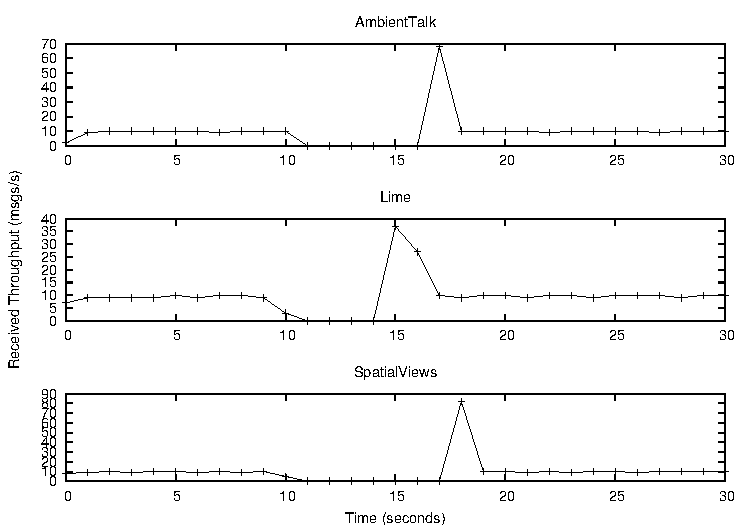
\includegraphics[scale = .70]{figures/disconnection.pdf}
\caption{Disconnection Recovery}
\label{fig:disconnection}
\end{figure}

\begin{figure}
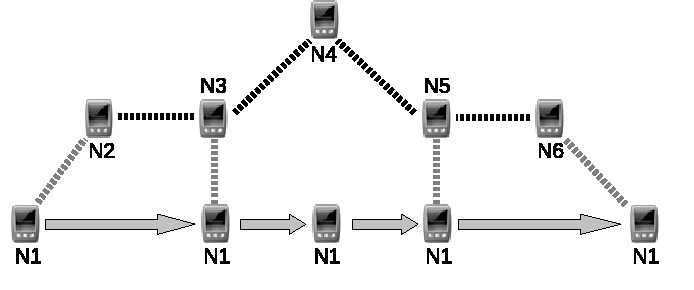
\includegraphics[scale = .70]{figures/network.pdf}
\caption{Simulated Mobility Scenario}
\label{fig:network}
\end{figure}

\begin{figure}
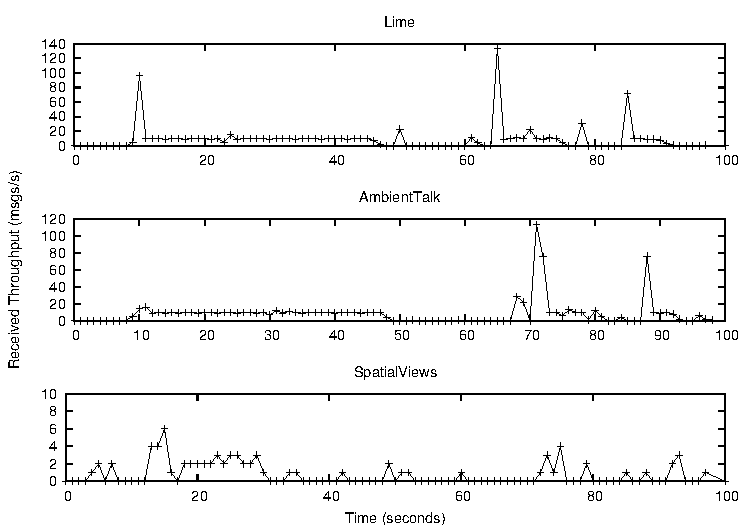
\includegraphics[scale = .70]{figures/mobility-results.pdf}
\caption{Client-Server Throughput with Mobility}
\label{fig:mobility-results}
\end{figure}

In order to isolate and examine disconnection recovery, a simpler experiment in a wired LAN was performed, still using the same client-server application. In this case, a 5 second disconnection was caused by turning the network interface off and then turning it back on. Each project reacted similarly, as shown in Figure~\ref{fig:disconnection} though LIME showed the fastest recovery time. Interestingly, SpatialViews exhibited delivery of buffered messages. As SpatialViews does not buffer messages itself, this buffering was the result of the operating system attempting to locate the remote node.

Using EXata, it was possible to evaluate the projects in a mobile environment which provided disconnections, routing changes, and multi-hop communication. For this experiment, the network layout and mobility pattern shown in Figure~\ref{fig:network} was used. Node 1 user the same client-server application as in the first experiment and is attempting to send messages to Node 4. The distance between the two nodes forces a multi-hop route through the intermediate nodes. Node 1 moves from left to right at a constant rate during a time period of 100 seconds. This experiment again measures message delivery rate. Results are shown in Figure~\ref{fig:mobility-results}. 

The large spikes for the AmbientTalk and LIME results indicate the delivery of buffered messages. For AmbientTalk, the sender did not begin until the receiver was discovered, while LIME began sending messages immediately. The flat part of the graphs indicates when Node 1 was in between Node 3 and Node 5 and was outside the range of both. SpatialViews did not perform well in this experiment because it lacks the sophisticated disconnection handling and message buffering of the other two experiments. Also, the code migration was difficult, more time consuming, and more susceptible to disconnections. As in the previous experiments, this demonstrates the difference between experiments using a wired LAN compared to a simulated wireless network. 